\documentclass[11pt]{article}
\usepackage[utf8]{inputenc}
\usepackage{amsmath}
\usepackage{amsfonts}
\usepackage{amssymb}
\usepackage{graphicx}
\usepackage[super]{nth}
\usepackage{amsthm}
\usepackage{bm}
\newtheorem{theorem}{Theorem}
\newtheorem{objective}{Objective}
\newtheorem{model}{Model}
\usepackage{xcolor}
\definecolor{light-gray}{gray}{0.95}
\newcommand{\code}[1]{\colorbox{light-gray}{\texttt{#1}}}
\usepackage{listings}
\usepackage{placeins}
\usepackage{enumitem}

\usepackage[authoryear]{natbib}

\lstset{language=R}


\makeatletter
\renewcommand{\maketitle}{
\begin{center}

\pagestyle{empty}

{\Large \bf \@title\par}
\vspace{1cm}

{\LARGE Marcel Gietzmann-Sanders}\\[1cm]

STAT651 - Statistical Theory I \\
University of Alaska Fairbanks


\end{center}
}\makeatother


\title{Homework 2}

\date{2025}
\setcounter{tocdepth}{2}
\begin{document}
\maketitle

\section{Question 1}

\subsection{a}

First: $A \cup B \subset A \cup (B \cap A^C)$

If $x \in A \cup B$ then $x \in A$ or $x \in B$. We can make these two options exclusive by saying that either $x\in A$ or $x \in B$ and $x\notin A$. The latter is equivalent to $x \in B \cap A^C$ as if $x \notin A$ then it follows that $x \in A^C$. If $x\in A$ then $x \in A \cup (B \cap A^C)$ and if $x \in B \cap A^C$ then $x \in A \cup (B \cap A^C)$ also. Therefore $\forall x \in A \cup B, x \in A \cup (B \cap A^C)$ and so $A \cup B \subset A \cup (B \cap A^C)$. \newline

Second: $A \cup (B \cap A^C) \subset A \cup B$

If $x \in A \cup (B \cap A^C)$ then $x\in A$ or $x \in B \cap A^C$. Due to the definition of an intersection if $x \in B \cap A^C$ then $x \in B$. If $x \in A$ then $x \in A \cup B$ and if $x \in B \cap A^C$ then $x\in B$ and so $x \in A \cup B$. Therefore $\forall x \in A \cup (B \cap A^C) , x \in A \cup B$ and so $A \cup (B \cap A^C) \subset A \cup B$. \newline

Given $A \cup B \subset A \cup (B \cap A^C)$ and $A \cup (B \cap A^C) \subset A \cup B$ it follows that $A \cup B = A \cup (B \cap A^C)$

\subsection{b}

First: $B \subset (B \cap A) \cup (B \cap A^C)$.

Assume an element $x\in B$ is not an element of either $A$ or $A^C$, then given the definition of complements $A \cup A^C=S$ where $S$ is all possible events, it follows that $x\notin S$. This is a contradiction as $x\in B \subset S$. Therefore $x\in A$ or $x\in A^C$. If $x\in B$ and $x\in A$ then $x \in B \cap A$ and therefore $x \in  (B \cap A) \cup (B \cap A^C)$. If $x\in B$ and $x\in A^C$ then $x \in B \cap A^C$ and therefore $x \in  (B \cap A) \cup (B \cap A^C)$. Thus if $x \in B$ then $x \in (B \cap A) \cup (B \cap A^C)$ and so $B \subset (B \cap A) \cup (B \cap A^C)$. \newline

Second: $(B \cap A) \cup (B \cap A^C) \subset B$.

If $x\in (B \cap A) \cup (B \cap A^C)$ then $x \in B \cap A$ or $x \in B \cap A^C$. If $x \in B \cap A$ then $x \in B$ and if $x \in B \cap A^C$ then $x\in B$. Therefore if $x\in (B \cap A) \cup (B \cap A^C)$ then $x\in B$ and $(B \cap A) \cup (B \cap A^C) \subset B$. \newline

Given $B \subset (B \cap A) \cup (B \cap A^C)$ and $(B \cap A) \cup (B \cap A^C) \subset B$ it follows that $B=(B \cap A) \cup (B \cap A^C)$.

\begin{figure}[h!] 
	\centering
  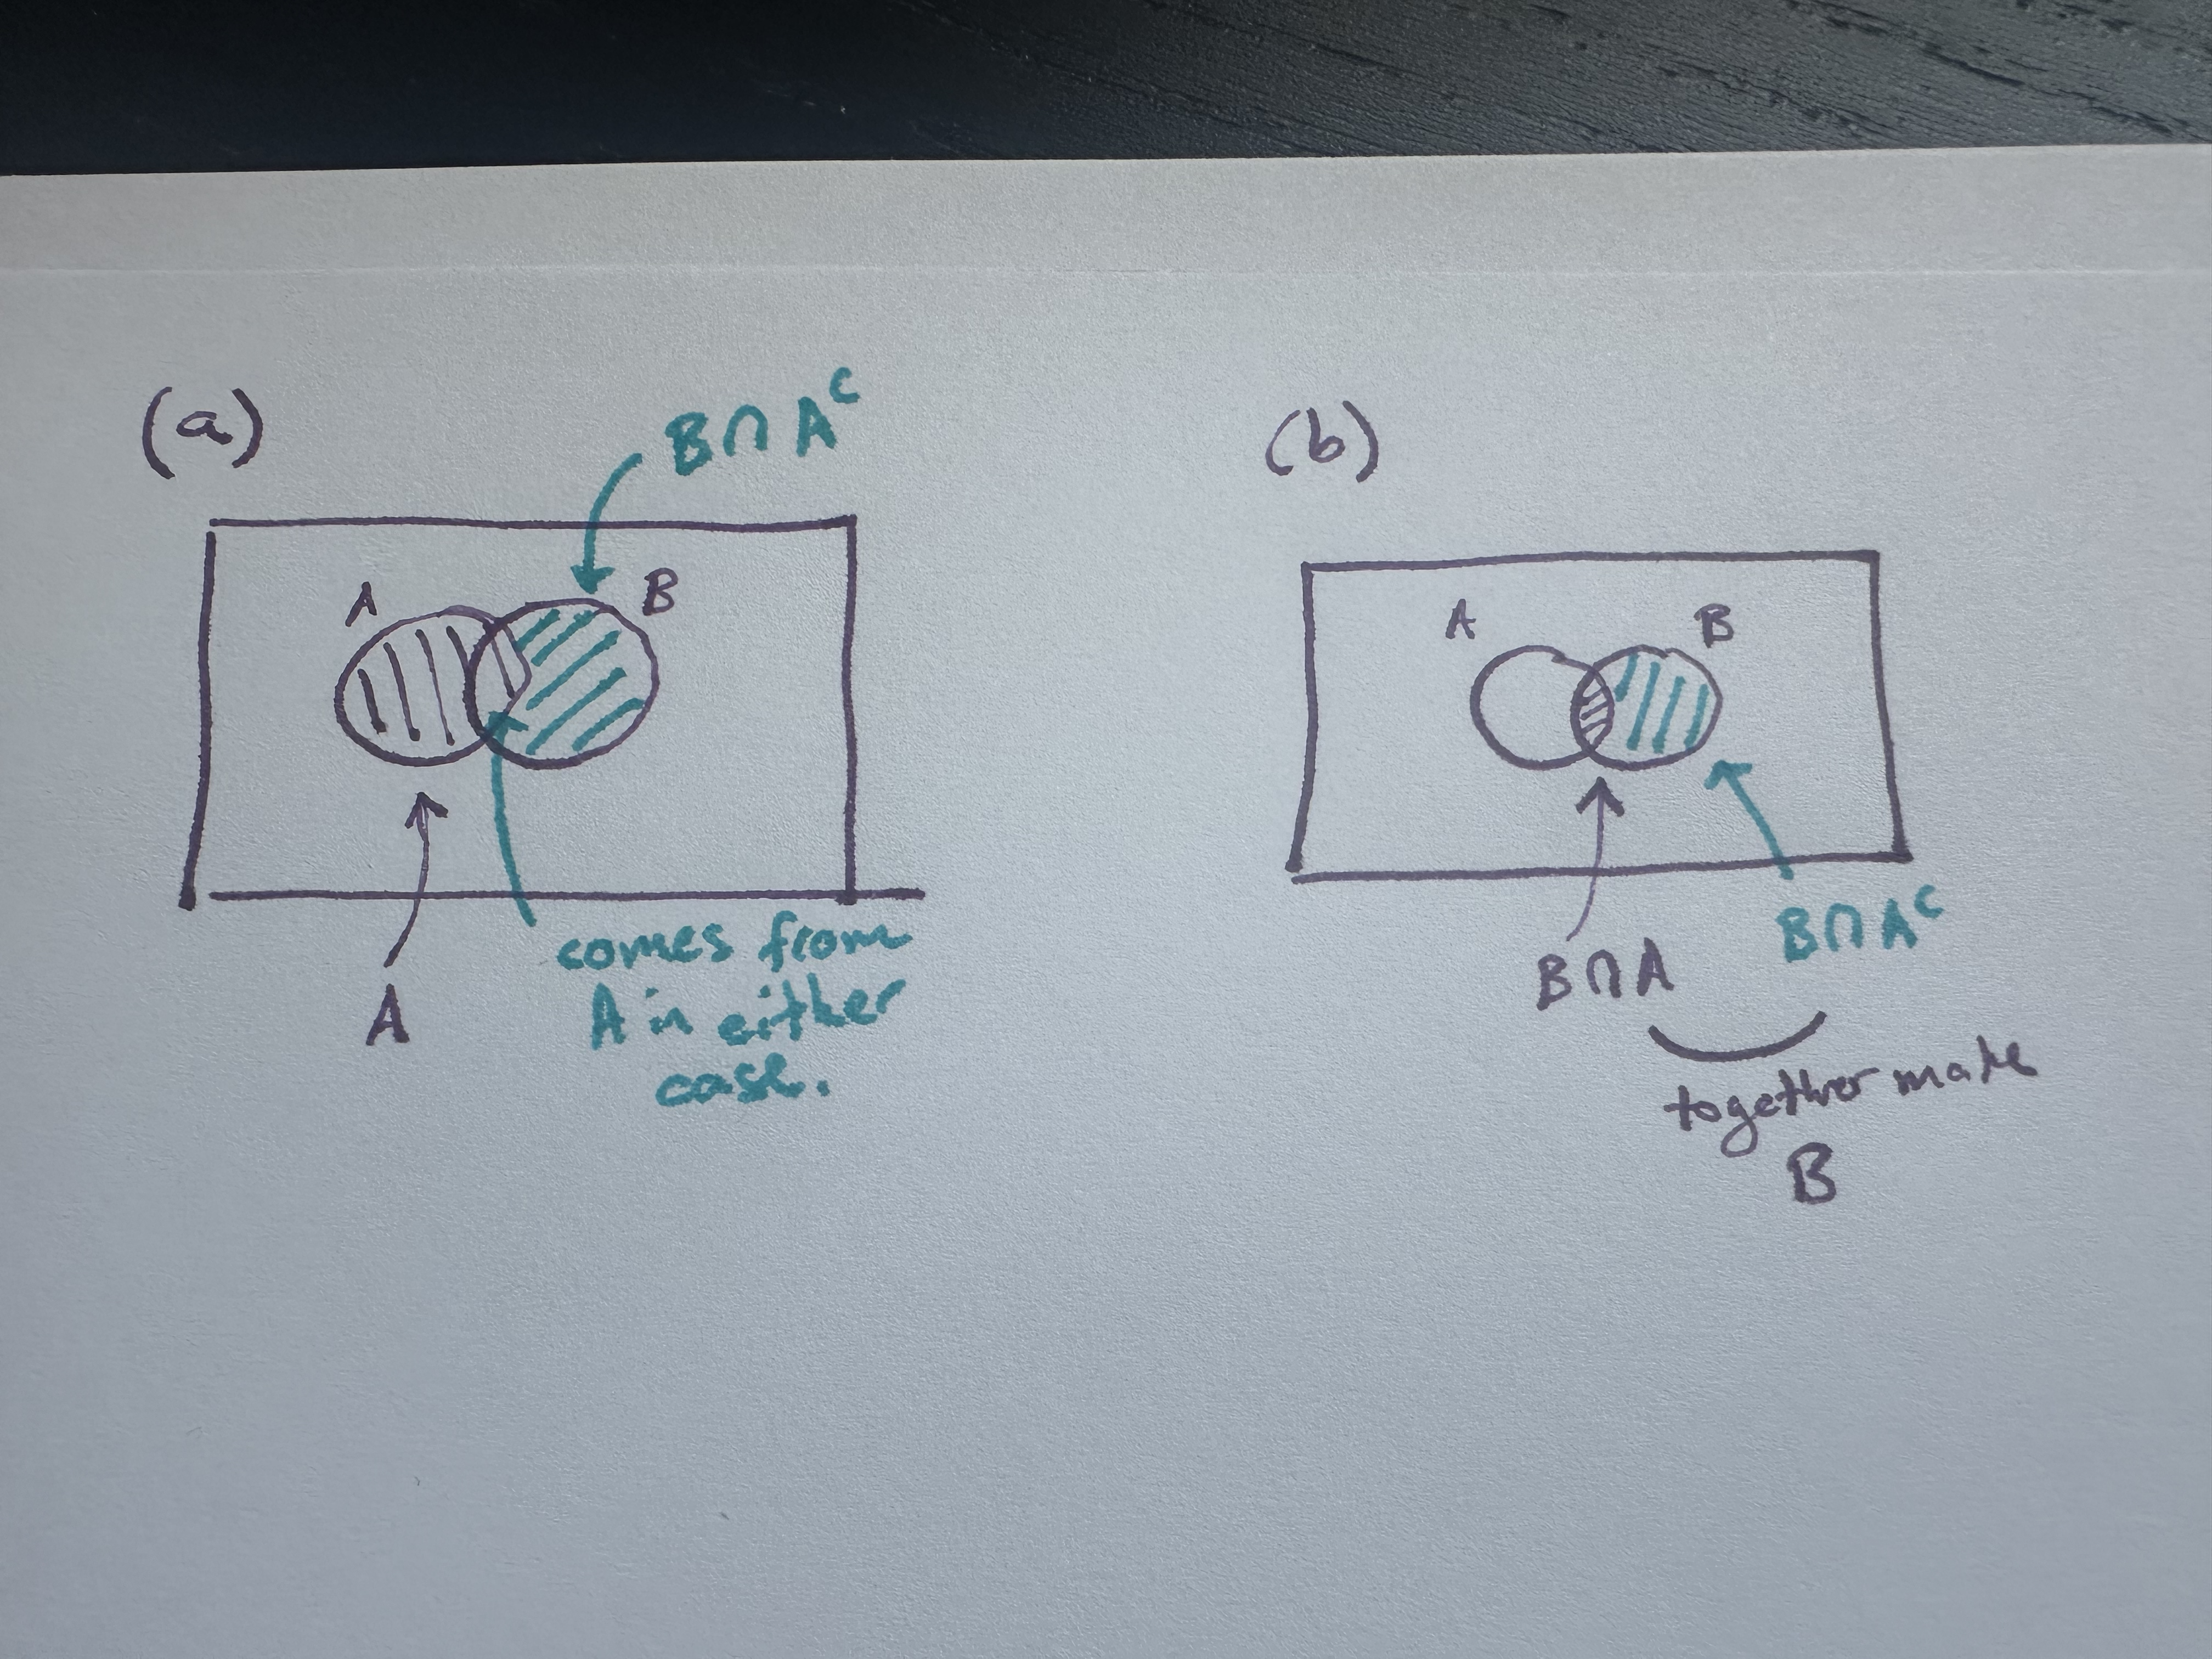
\includegraphics[height=100mm]{illustrate.png}
  \label{fig:illustrate}
\end{figure}

\FloatBarrier
\newpage

\section{Question 2}

\begin{enumerate}[label=\alph*]
\item We're interested here in $P(A\cup B)$. $A \cup B = (A \cap B^C) \cup (B \cap A^C) \cup (A \cap B)$. All sets on the right hand side have zero intersection with one another. Therefore $P(A\cup B) = P(A \cap B^C) + P(B \cap A^C) + P(A \cap B)$. By similar reasoning $P(A) = P(A\cap B^C) + P(A \cap B) \rightarrow P(A \cap B^C) = P(A) - P(A \cap B)$ and $P(B) = P(B \cap A^C) + P(A \cap B) \rightarrow P(B \cap A^C) = P(B) - P(A \cap B)$. Therefore by substitution we get $P(A \cup B) = P(A) + P(B) - P(A \cap B)$. 
\item Here we're interested in $P((A\cap B^C) \cup (B \cap A^C))$ which, using the above, is $P(B) + P(A) - 2P(A \cap B)$. 
\item Same as (a) 
\item What we are interested is the complement of $A \cap B$. Therefore our probability is just $1 - P(A \cap B)$. 
\end{enumerate}

\section{Question 3}

\begin{enumerate}[label=\alph*]
\item a U.S birth results in identical, female twins. 
\item $P(A\cap B \cap C) = (1/90)(1/3)(1/2) = 1/540$. 
\end{enumerate}

\section{Question 4}

No. For $B$ and $A$ to be disjoint, $A \subset B^C$. This would mean $P(A) \leq P(B^C)$ but in our case $1/3$ is greater than $1/4$. So $B^C$ cannot contain $A$ and so $A$ and $B$ cannot be disjoint. 

\newpage

\section{Question 5}

(a) 

\begin{figure}[h!] 
	\centering
  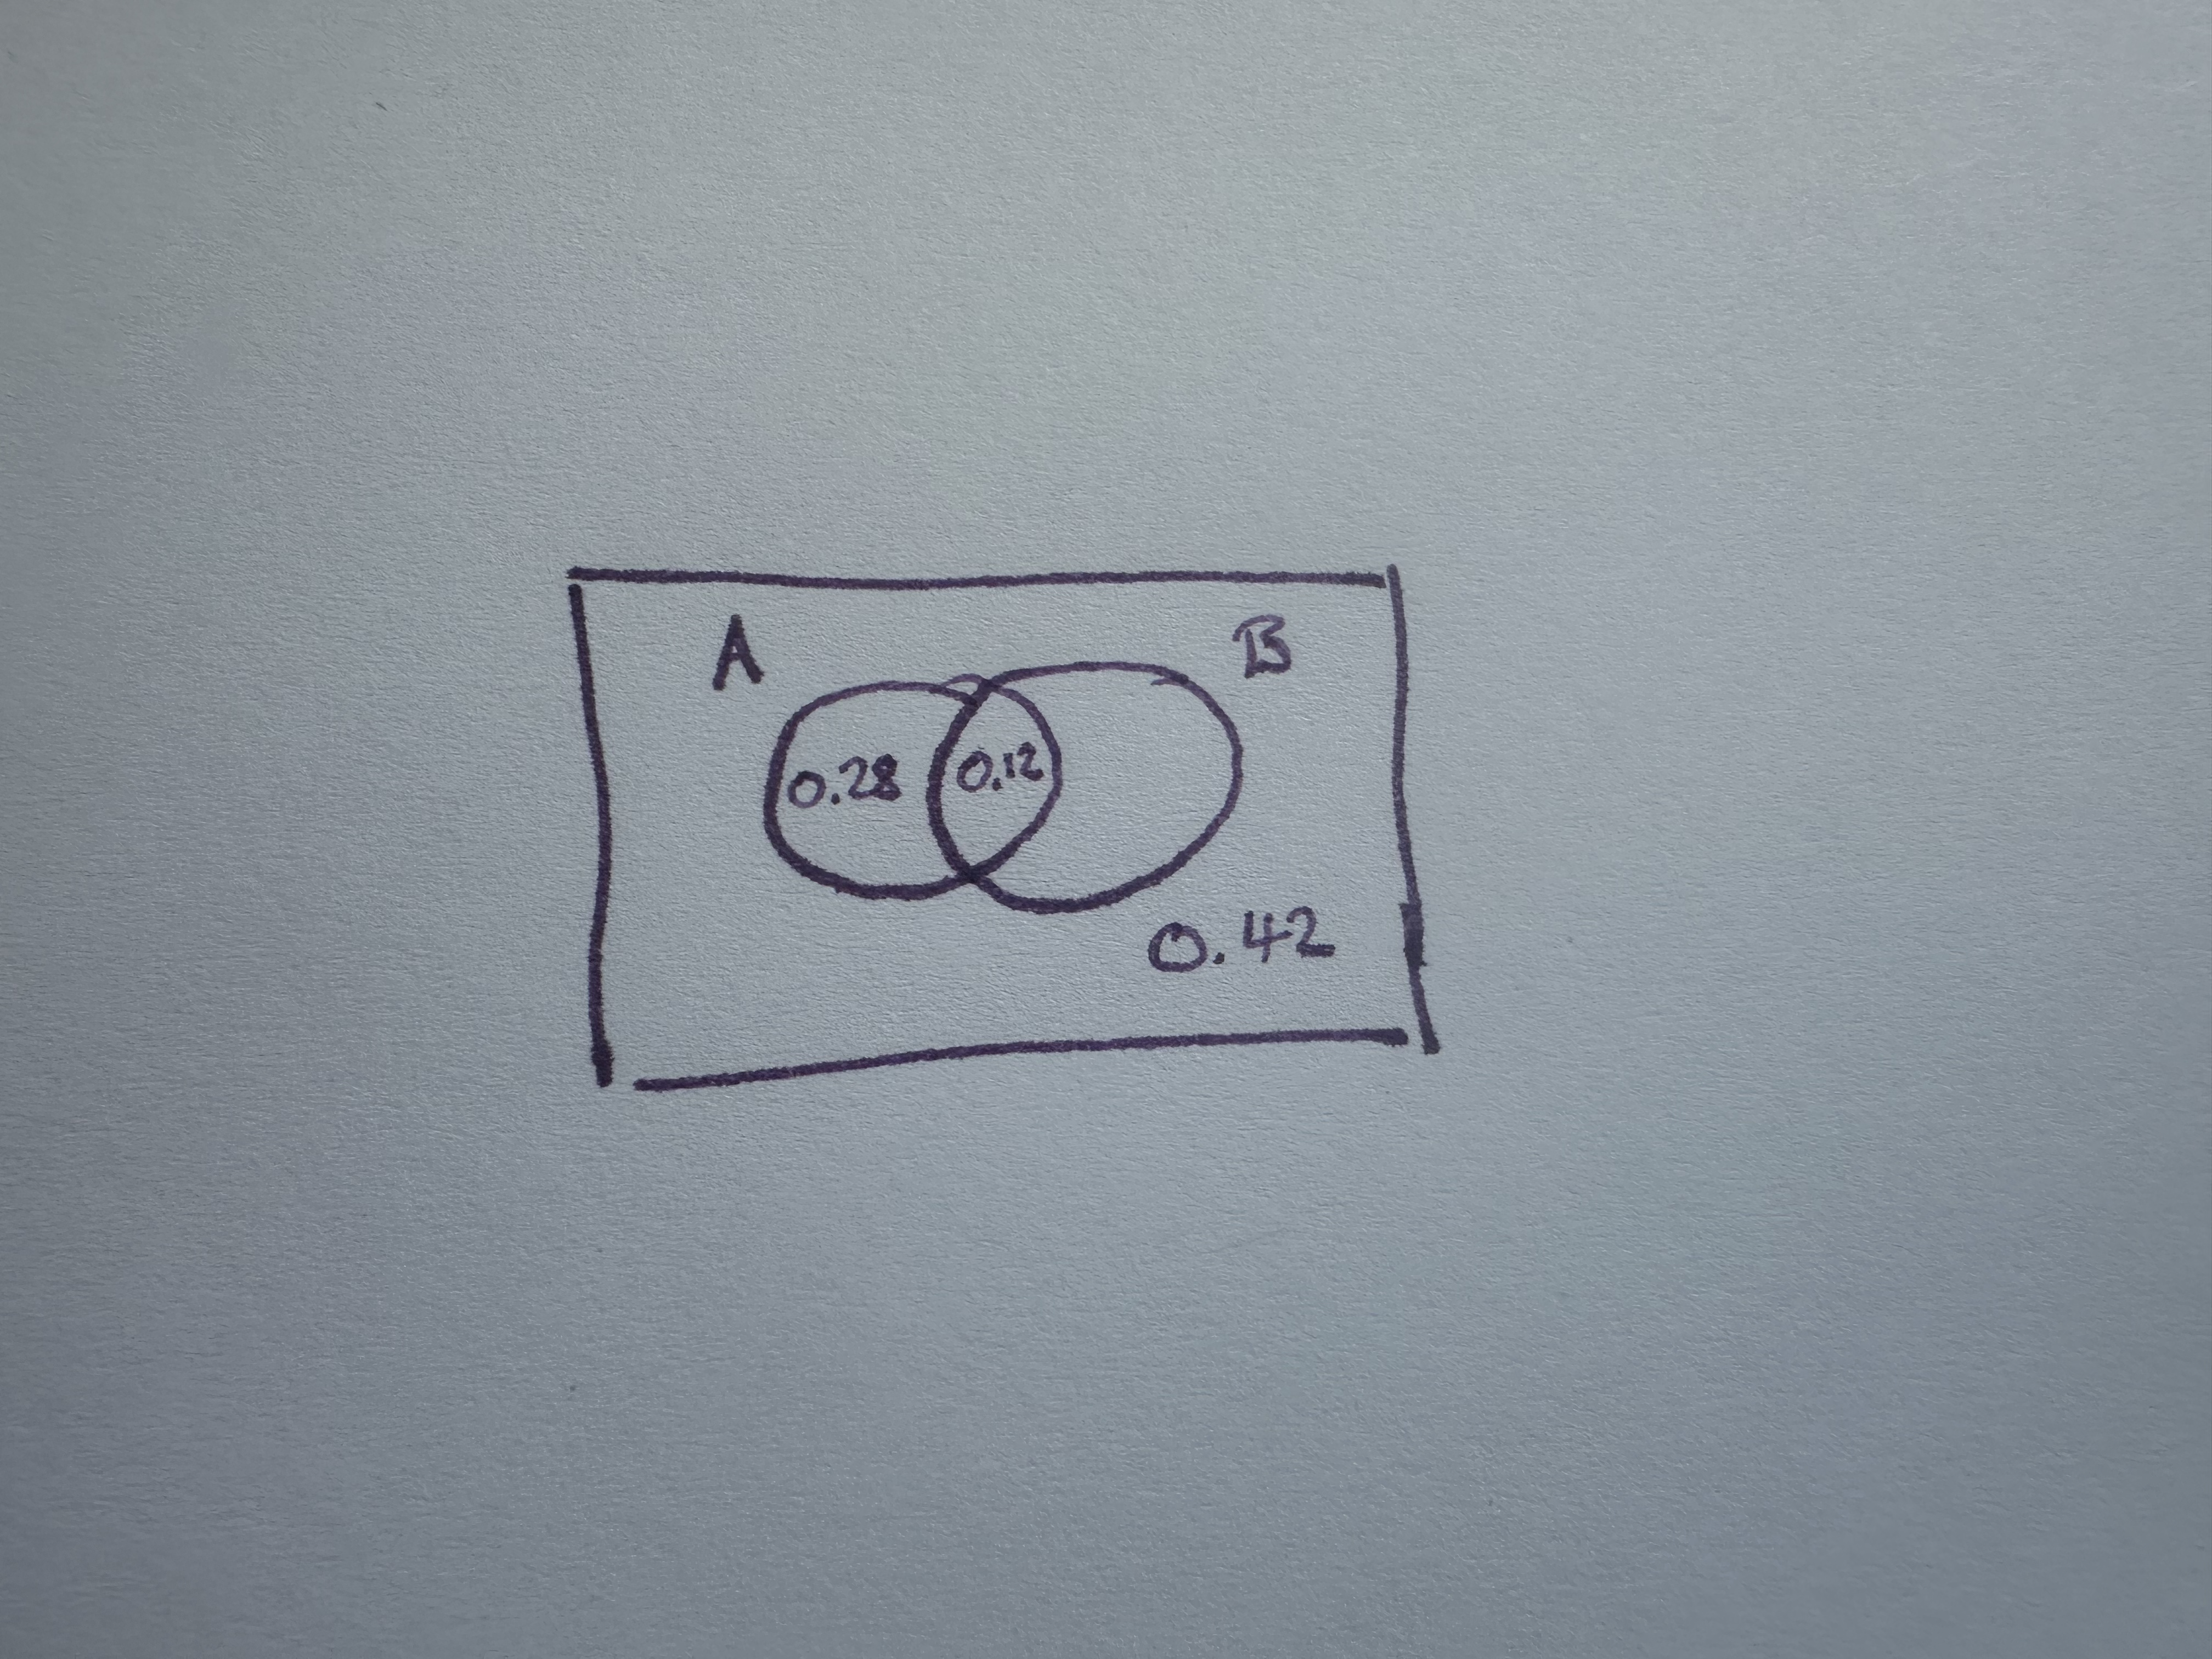
\includegraphics[height=100mm]{venn.png}
  \label{fig:venn}
\end{figure}

\FloatBarrier

(b) $P(A) = 0.12 + 0.28 = 0.4$, $P(B) = 1 - 0.42 - 0.28 = 0.3$, $P(A\cup B) = 1 - 0.42 = 0.58$, $P(A^C \cap B) = 0.3 - 0.12 = 0.18$. 

\newpage

\section{Question 6}

\subsection{a}

If we put our coins in order of value our outcomes look like $HHHT$, $THTH$, $TTTT$. Given each coin has 2 options we have $2^4=16$ elements in $S$. Now the elements of our sigma algebra will be sets of size 0 - 16 that are combinations of the elements of $S$. That is we have:

$$\sum_{i=0}^{16} {16 \choose i}=65,536$$

elements in our sigma algebra. 

\subsection{b}

In this case our outcomes look like 0H's, 1H, 2H's, ... 4H's (once we know the number of heads we know the number of tails). Therefore there are 5 elements in $S$ and our sigma algebra will constitute the sets of size 0 - 5 that are combinations of those elements. That is we have:

$$\sum_{i=0}^{5} {5 \choose i}=32$$

elements in our sigma algebra.

\subsection{c}

Here we have 0H's, 1H, or 2H's for each group. And we have two groups so there are $3^2=9$ distinct elements in $S$. Using the same reasoning as for the other questions we have:

$$\sum_{i=0}^{9} {9 \choose i}=512$$

elements in our sigma algebra.

\subsection{d}

Whether they are called penny, nickle, dime and quarter or first, second, third, and fourth shouldn't matter. The answer is the same as for (a) - 65,536.

\section{Question 7} 

\begin{figure}[h!] 
	\centering
  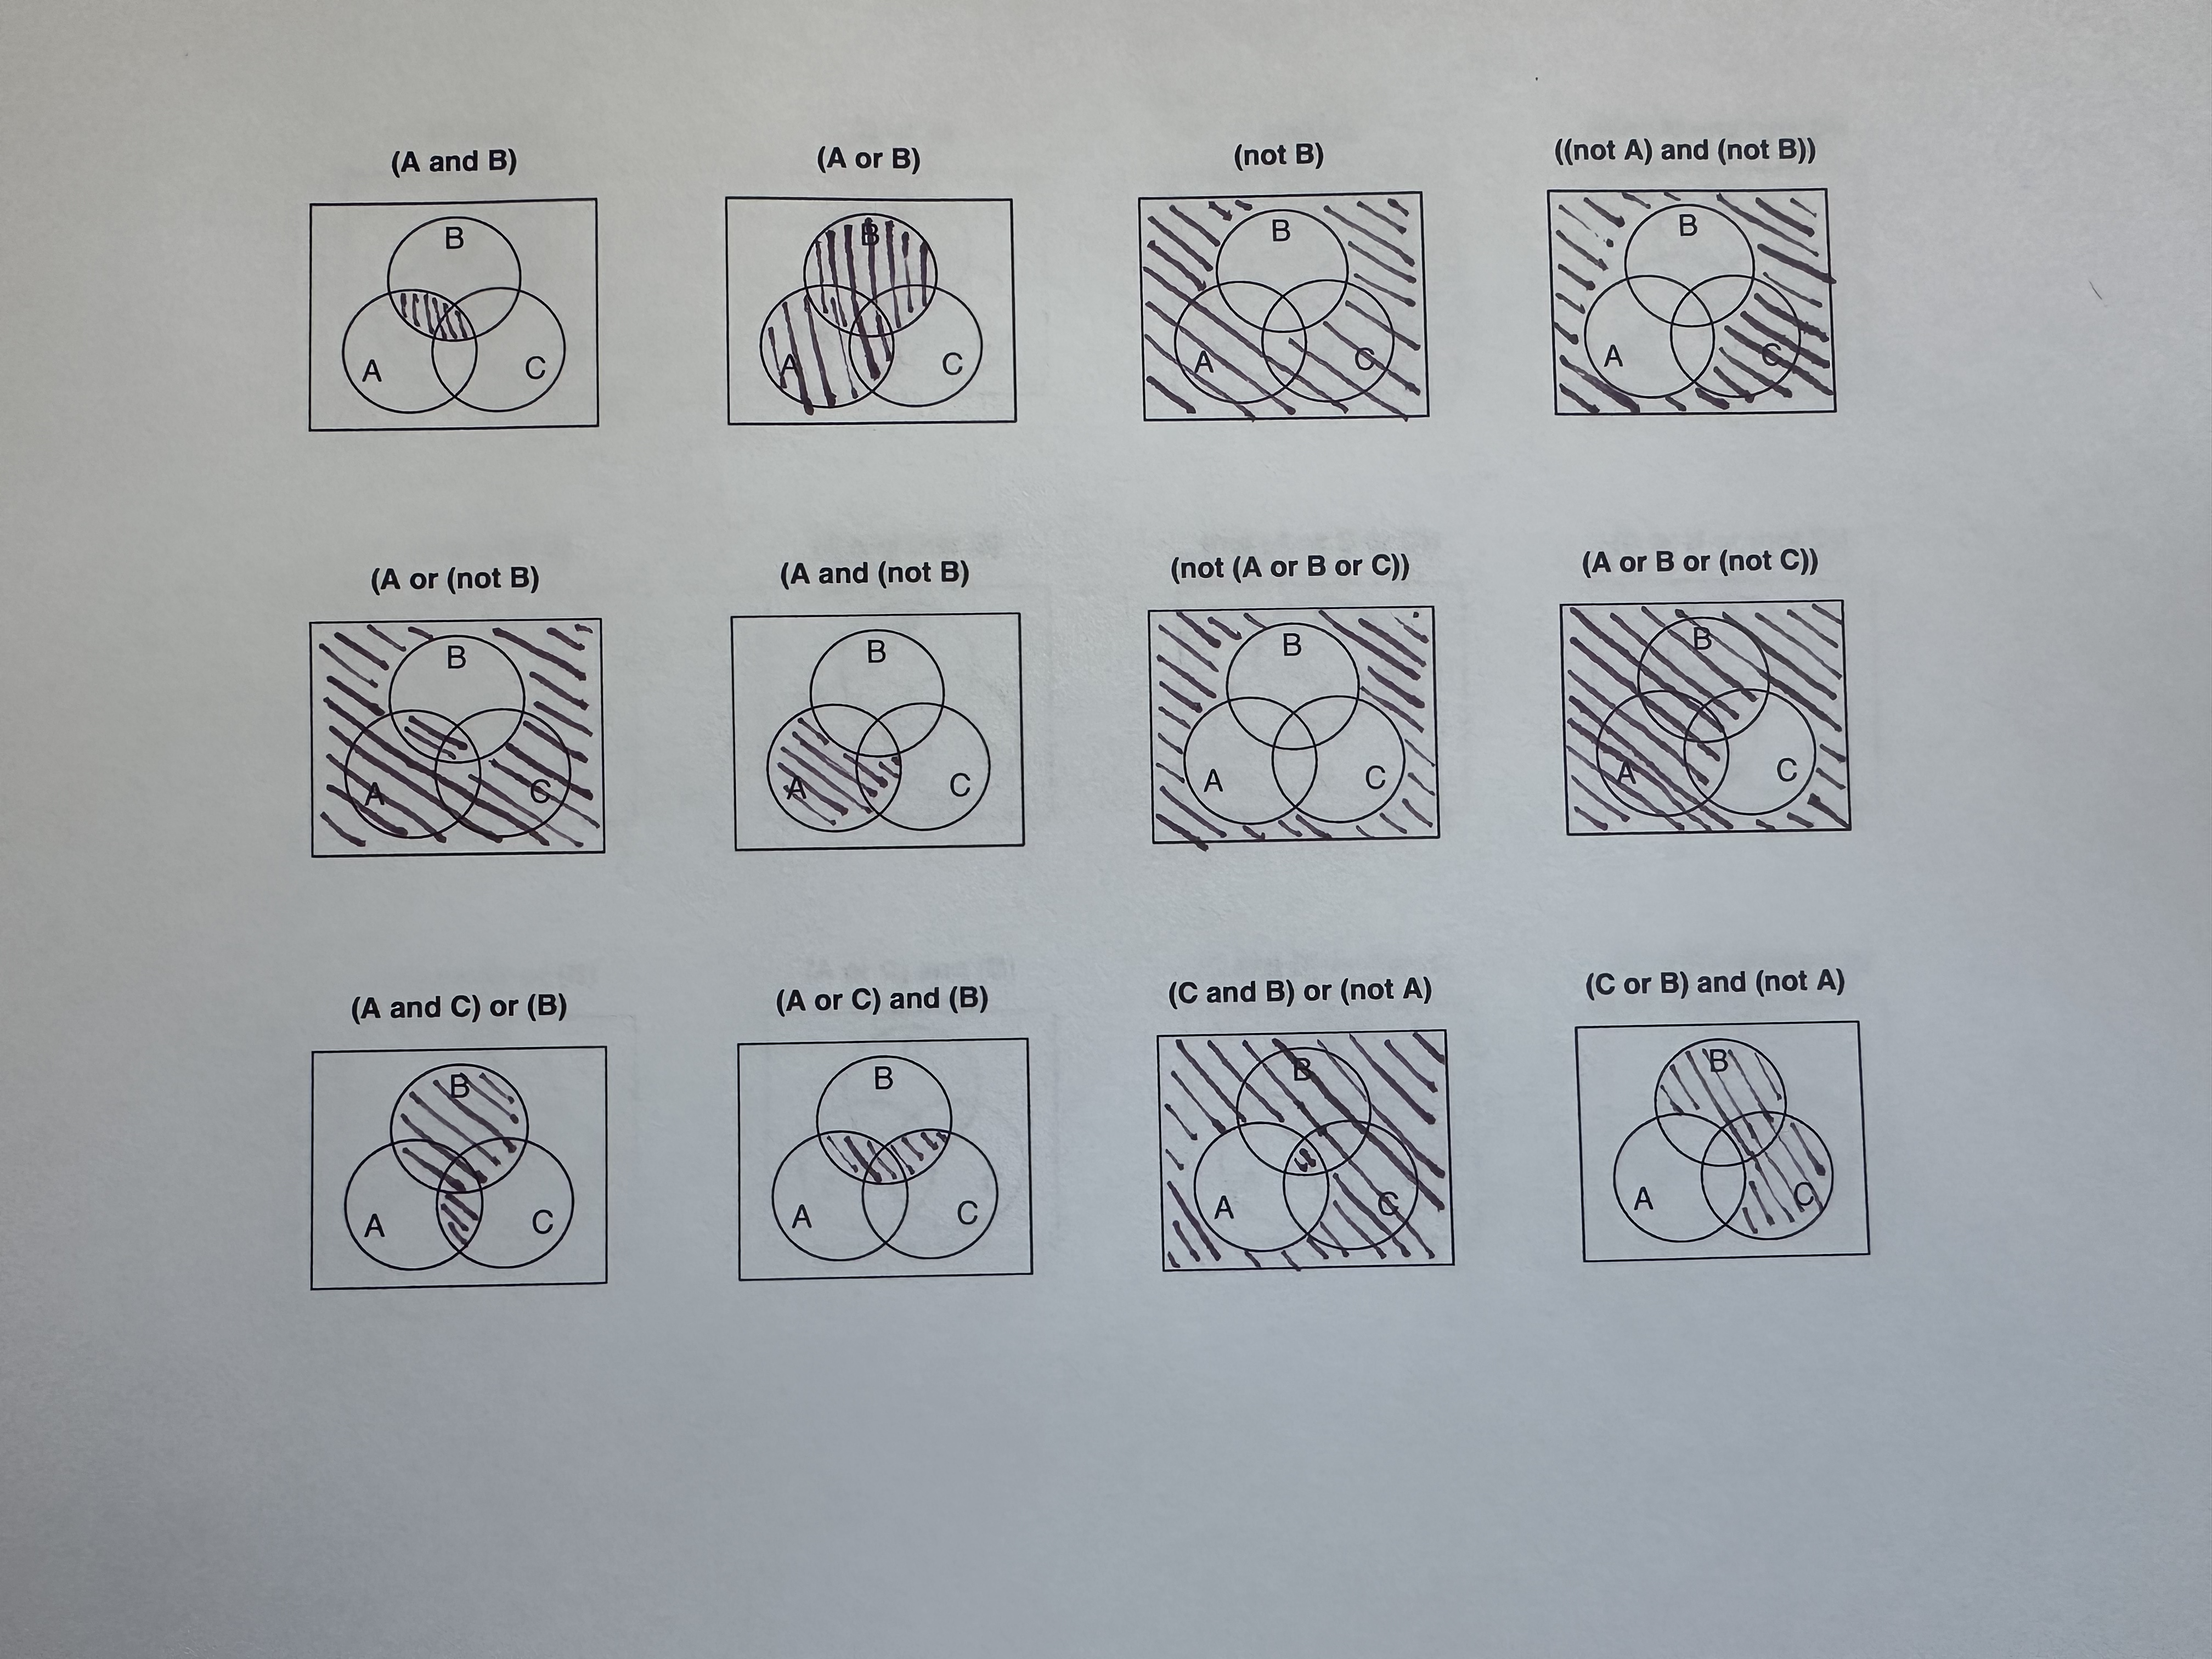
\includegraphics[height=100mm]{shading.png}
  \label{fig:shading}
\end{figure}

\FloatBarrier


\end{document}